% id: 0328
% book: RPM 중3-2 수학 · 03 원과 직선
% section: 유형 16 원에 외접하는 사각형의 성질 (2)
% figure: crop:fig-0328.png
% answer: $5\,\mathrm{cm}$
% answer_source: 답지
% variant_level: 0 (원본 전사)
% 이 파일은 build.mjs 가 items.json 에서 만든다. 고칠 때는 items.json 을 고친다.
\dmkichul{RPM 중3-2 수학 0328번 · 54쪽}
\noindent\begin{minipage}[t]{0.58\linewidth}\vspace{0pt}\raggedright 오른쪽 그림과 같이 $\square\pt{ABCD}$는 원~$\pt{O}$에 외접한다. $\angle\pt{C}=\angle\pt{D}=90^\circ$이고, $\seg{BC}=6\,\mathrm{cm}$, $\seg{CD}=4\,\mathrm{cm}$일 때, $\seg{AB}$의 길이를 구하시오.\end{minipage}\hfill\begin{minipage}[t]{0.4\linewidth}\vspace{0pt}\centering 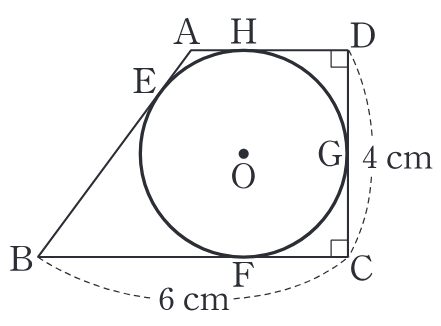
\includegraphics[width=105.8pt]{figures/fig-0328.png}\end{minipage}\par
